\section{Matchings in Bipartite Graphs}

Hypergraphs came up in \Cref{Ch1:Def:Hypergraph} as the setting in which the coloring question gets hard, and \Cref{Ch1:CH} set them aside again once it had its answer. The first thing this chapter asks of them is this: given a hypergraph, can we pick one vertex out of each edge, all of them different? Getting to the answer means first noticing that a hypergraph, a $0,1$ matrix and a bipartite graph are three views of the same data.

\subsection{Adjacency Matrices}

We can represent the data of a hypergraph $H$ in a matrix, known as the adjacency matrix.

% [CORRECTED] was: "with $n$ vertices and $m$ hyper-edges, then" --- a hypergraph is a collection of subsets and carries
% no ordering of either, so without one the recipe names $n! m! / \abs{\operatorname{Aut}(H)}$ matrices rather than one.
\begin{boxdefinition}[Adjacency Matrix]
    If $H$ is a hypergraph with $n$ vertices and $m$ hyper-edges, both taken in some fixed order, then the adjacency matrix of $H$, denoted $\Adj(H)$, is the unique $n \times m$ matrix $\parenth{a_{ij}}$ where
    \begin{align*}
        a_{ij} =
        \begin{cases}
            1 & \text{ if vertex $i$ lies in hyper-edge $j$} \\
            0 & \text{ otherwise}
        \end{cases}
    \end{align*}
\end{boxdefinition}

Here are some examples of constructing adjacency matrices.

\begin{boxexample}[Some Adjacency Matrices of Hypergraphs] \hfill
    \begin{enumerate}
        \item Consider the hypergraph
        \begin{center}
            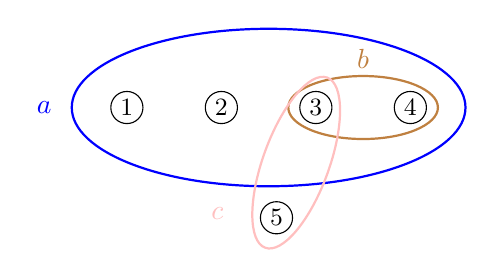
\begin{tikzpicture}
                \draw[thick, blue] (1.8, 0) ellipse (2.5 and 1.0);
                \draw[thick, brown] (3.0, 0) ellipse (0.95 and 0.4);
                \draw[thick, pink, rotate around = {70:(2.15, -0.7)}] (2.15, -0.7) ellipse (1.15 and 0.42);
                \node[blue] at (-1.05, 0) {$a$};
                \node[brown] at (3.0, 0.62) {$b$};
                \node[pink] at (1.15, -1.35) {$c$};
                \foreach \i/\x in {1/0, 2/1.2, 3/2.4, 4/3.6}{
                    \node[circle, draw = black, fill = white, inner sep = 1.5pt, font = \small] at (\x, 0) {$\i$};
                }
                \node[circle, draw = black, fill = white, inner sep = 1.5pt, font = \small] at (1.9, -1.4) {$5$};
            \end{tikzpicture}
        \end{center}
        Its adjacency matrix is
        \begin{align*}
            \begin{bmatrix}
                1 & 0 & 0 \\
                1 & 0 & 0 \\
                1 & 1 & 1 \\
                1 & 1 & 0 \\
                0 & 0 & 1
            \end{bmatrix}
        \end{align*}

        \item Consider the hypergraph
        % [CORRECTED] was the $3 \times 5$ matrix with rows (1 1 1 1 0), (0 0 1 1 0), (0 0 1 0 1) --- its first two
        % columns are equal, and a hypergraph is a collection of subsets, so distinct hyper-edges give distinct
        % columns and no five-edge hypergraph has that matrix. The duplicate column is dropped. So the correspondence
        % claimed after this example runs between hypergraphs and those $0,1$ matrices whose columns are distinct,
        % up to permutation of the rows and of the columns.
        \begin{align*}
            \begin{bmatrix}
                1 & 1 & 1 & 0 \\
                0 & 1 & 1 & 0 \\
                0 & 1 & 0 & 1
            \end{bmatrix}
        \end{align*}
        Reading the columns off one at a time, this is the hypergraph on three vertices with the four hyper-edges $f_1 = \set{1}$, $f_2 = \set{1, 2, 3}$, $f_3 = \set{1, 2}$ and $f_4 = \set{3}$.
        \begin{center}
            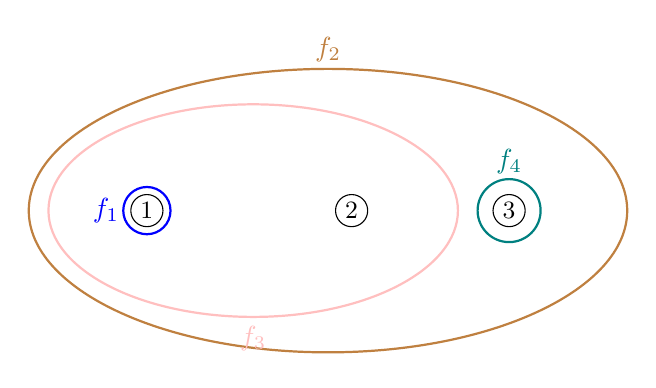
\begin{tikzpicture}
                \draw[thick, brown] (2.3, 0) ellipse (3.8 and 1.8);
                \draw[thick, pink] (1.35, 0) ellipse (2.6 and 1.35);
                \draw[thick, blue] (0, 0) circle (0.3);
                \draw[thick, teal] (4.6, 0) circle (0.4);
                \node[brown] at (2.3, 2.05) {$f_2$};
                \node[pink] at (1.35, -1.62) {$f_3$};
                \node[blue] at (-0.52, 0) {$f_1$};
                \node[teal] at (4.6, 0.62) {$f_4$};
                \foreach \i/\x in {1/0, 2/2.6, 3/4.6}{
                    \node[circle, draw = black, fill = white, inner sep = 1.5pt, font = \small] at (\x, 0) {$\i$};
                }
            \end{tikzpicture}
        \end{center}
    \end{enumerate}
\end{boxexample}

It turns out that there is not just a correspondence between hypergraphs and $0,1$ adjacency matrices, we can also complete the trifecta with bipartite graphs.

\begin{figure}[H]
    \centering
    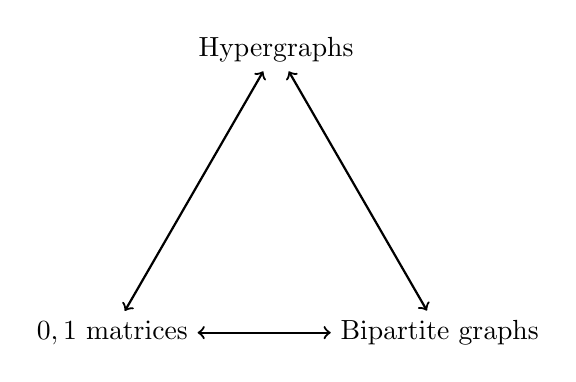
\begin{tikzpicture}
        \node[align = center] (hyp) at (90:2.4) {Hypergraphs};
        \node[align = center] (mat) at (210:2.4) {$0,1$ matrices};
        \node[align = center] (bip) at (330:2.4) {Bipartite graphs};
        \draw[<->, thick] (hyp) -- (mat);
        \draw[<->, thick] (mat) -- (bip);
        \draw[<->, thick] (bip) -- (hyp);
    \end{tikzpicture}
\end{figure}

The bipartite graph attached to $H$ has the vertices of $H$ on one side and the hyper-edges of $H$ on the other, with $v$ joined to $f$ exactly when $v \in f$, which is to say exactly when the adjacency matrix has a $1$ in position $(v, f)$.

\subsection{Hall's Marriage Theorem}

Recall, now, the most important result about bipartite graphs.

% [CORRECTED] was: "$\Gamma(S) = \setst{v \in B}{\exists u \in A \st u \sim v}$" --- quantified over $A$, $\Gamma$ does not
% depend on its argument, so the condition collapses to $\abs{\Gamma(A)} \geq \abs{A}$ and the theorem is false.
% [CORRECTED] was: "Given a bipartite graph with parts $A$ and $B$" --- with $A$ infinite the "if" direction is false:
% join $a_0$ to every $b_i$ and $a_i$ to $b_i$ alone, and Hall's condition holds while $a_0$ has nowhere to go. The
% induction below is on $\abs{A}$ and needs it. $B$ is never counted, so it may stay arbitrary.
\begin{boxtheorem}[Hall's Marriage Theorem] \label{Ch2:Thm:Hall}
    Given a bipartite graph with parts $A$ and $B$, with $A$ finite, there is a complete matching of $A$ iff $\forall S \subseteq A$,
    \begin{align*}
        \abs{\Gamma(S)} \geq \abs{S}
    \end{align*}
    where $\Gamma(S) = \setst{v \in B}{\exists u \in S \st u \sim v}$.
\end{boxtheorem}
\begin{iffproof}
    \onlyifdir Let $M$ be a complete matching of $A$ and let $S \subseteq A$. The partners under $M$ of the elements of $S$ are $\abs{S}$ distinct vertices of $B$, each adjacent to something in $S$, so $\Gamma(S)$ has at least $\abs{S}$ elements.

    \ifdir We induct on $\abs{A}$. If $\abs{A} = 1$, then Hall's condition applied to $A$ itself says that the one vertex of $A$ has a neighbor, and matching it to one is a complete matching. So suppose $\abs{A} > 1$, and let's do some casework.
    \begin{itemize}
        \item \underline{Case 1:} Assume that in fact, $\forall S \subsetneq A$ nonempty, $\abs{\Gamma(S)} \geq \abs{S} + 1$. Arbitrarily match some pair: pick any $a \in A$ and any $b \in \Gamma(\set{a})$, which is nonempty by hypothesis. After deleting this edge---and with it the vertices $a$ and $b$ and every other edge at either of them---the rest satisfies the desired result, since a nonempty $T \subseteq A \setminus \set{a}$ is a nonempty proper subset of $A$ and so had at least $\abs{T} + 1$ neighbors to begin with, of which deleting $b$ can take away only one. What is left has $\abs{A} - 1$ vertices on the left, so we are done by induction: it has a complete matching of $A \setminus \set{a}$, and adding the edge $ab$ to that matching completes it to one of $A$.

            \item \underline{Case 2:} Now assume the opposite, ie, that $\exists S \subsetneq A$ nonempty such that $\abs{\Gamma(S)} = \abs{S}$. We will apply induction again, on $\abs{A}$ as before.

            % [CORRECTED] was: "by both the definition of $\Gamma$ and the fact that they're of equal cardinality" --- equal
            % cardinality does not on its own give a matching; what does is the induction hypothesis.
            If we restrict our attention to $S$, obviously we have a perfect matching between $S$ and $\Gamma(S)$: every $T \subseteq S$ has $\Gamma(T) \subseteq \Gamma(S)$, so the graph they span satisfies Hall's condition and induction gives a complete matching of $S$, which the fact that they're of equal cardinality makes perfect. (There may be more than one, but there is one.)

            % [CORRECTED] was: "any bipartite graph structure on $A'$ and $B'$ also has a perfect matching" --- it is the
            % induced structure and no other, and $\abs{B'} - \abs{A'} = \abs{B} - \abs{A}$ need not be $0$, so the matching
            % is complete rather than perfect.
            Define $A' = A \setminus S$, $B' = B \setminus \Gamma(S)$. We claim that the bipartite graph induced on $A'$ and $B'$ also has a complete matching of $A'$, in which case we'd be done (by induction).

            % Not from the lecture: the verification of Hall's condition on A' and B' below, and
            % the assembly of the two matchings, were supplied to close the gap the lecture left here.
            Writing $\Gamma'$ for the neighborhood taken in that smaller graph, we have $\Gamma'(T) = \Gamma(T) \setminus \Gamma(S)$ for every $T \subseteq A'$, and $\Gamma(S \cup T) = \Gamma(S) \cup \Gamma(T)$ as it does for any two sets, so
            \begin{align*}
                \abs{\Gamma'(T)} = \abs{\Gamma(S) \cup \Gamma(T)} - \abs{\Gamma(S)} = \abs{\Gamma(S \cup T)} - \abs{S} \geq \abs{S \cup T} - \abs{S} = \abs{T}
            \end{align*}
            where the inequality is Hall's condition applied to $S \cup T$, and the last step is that $T \subseteq A'$ is disjoint from $S$. (If $\Gamma(T)$ is infinite the display needs no reading at all: $\Gamma(S)$ is finite, so $\Gamma'(T)$ is infinite and certainly at least $\abs{T}$.) So the smaller graph satisfies Hall's condition, and $\abs{A'} < \abs{A}$ because $S$ is nonempty, so induction gives a complete matching of $A'$ into $B'$. That matching touches no vertex of $S$ and no vertex of $\Gamma(S)$, so laying it alongside the matching of $S$ onto $\Gamma(S)$ gives a complete matching of $A$.
    \end{itemize}
\end{iffproof}

% [CORRECTED] was: "a collection $x_1, \ldots, x_m$ such that $x_i \in f_i$" --- without distinctness the criterion below
% is false, and it is distinctness that corresponds to a matching under Hall.
% [CORRECTED] was: "for any collection of hyper-edges", with $\calC$ ranging over the whole of $\H$ --- on that reading the
% ``iff'' is false. Take $\H = \set{\set{1}, \set{2}, \set{1, 2}}$ with $f_1 = \set{1}$ and $f_2 = \set{2}$: representatives
% exist, while $\calC = \H$ gives $2 < 3$. Hall applied to the bipartite graph on the indices $1, \ldots, m$ delivers the
% condition for subcollections of the $f_i$ and for nothing else; the edges of $\H$ outside the $f_i$ are not in that graph.
Given a hypergraph $H$, a family of distinct representatives is a collection of distinct $x_1, \ldots, x_m$ such that $x_i \in f_i$, where we have distinct hyper-edges $f_1, \ldots, f_m$ in $\H$. Such a collection exists iff for any subcollection $\calC$ of $f_1, \ldots, f_m$,
\begin{align*}
    \abs{\bigcup_{f \in \calC} f} \geq \abs{\calC}
\end{align*}
In other words, the number of vertices in all the edges in the collection should be at least the number of edges in the collection. This is what Hall's Marriage Theorem tells us about hypergraphs.

% [CORRECTED] was: "We can, in fact, prove an even stronger statement than Hall." --- the result below is a corollary
% of Hall: its proof verifies Hall's condition and then cites it, and it applies to strictly fewer graphs.
Hall's condition asks something of every subset of $A$, which is a lot to check. There is a consequence of it that only asks about degrees.

% [CORRECTED] was: "with $d_2 \leq d_1$" --- $d_1 = d_2 = 0$ satisfies that, and an edgeless graph with $A$ nonempty has
% no complete matching. The proof divides by $d_2$, so $d_2 \geq 1$ is what it uses.
\begin{boxtheorem} \label{Ch2:Cor:Biregular}
    If $G$ is a bipartite graph with parts $A$ and $B$, if all degrees in $A$ are $d_1$ and all degrees in $B$ are $d_2$, with $1 \leq d_2 \leq d_1$, then there is a complete matching of $A$.
\end{boxtheorem}

Such a graph is a good deal more rigid than a bipartite graph with Hall's condition alone; here is one with $d_1 = 4$ and $d_2 = 2$.

\begin{figure}[H]
    \centering
    \begin{tikzpicture}
        \bipartiteparts{3}{6}
        \foreach \i/\j in {1/1, 1/2, 1/3, 1/4, 2/3, 2/4, 2/5, 2/6, 3/5, 3/6, 3/1, 3/2}{
            \draw (A\i) -- (B\j);
        }
        \node[anchor = south] at (0, 1.5) {$A$};
        \node[anchor = south] at (3, 2.55) {$B$};
    \end{tikzpicture}
\end{figure}

\begin{proof}
    Given a set $S \ssq A$, there are $d_1 \abs{S}$ edges coming out of $S$ and going to the right. Each vertex of $\Gamma(S)$ absorbs at most $d_2$ of them, so
    \begin{align*}
        \abs{\Gamma(S)} \geq \frac{d_1\abs{S}}{d_2} \geq \abs{S}
    \end{align*}
    so we can just apply \Cref{Ch2:Thm:Hall}.
\end{proof}
